\documentclass[11pt]{article}
% Shared preamble for the notes in this repository. pdfLaTeX, TeX Live 2024 or later.
\usepackage[a4paper,margin=2.6cm]{geometry}
\usepackage[T1]{fontenc}
\usepackage{lmodern}
\usepackage{microtype}
\usepackage{amsmath,amssymb,amsthm}
\usepackage{graphicx}
\usepackage{booktabs}
\usepackage{enumitem}
\usepackage[dvipsnames]{xcolor}
\usepackage[hidelinks]{hyperref}
\hypersetup{colorlinks=true,linkcolor=MidnightBlue,citecolor=MidnightBlue,urlcolor=MidnightBlue}
\graphicspath{{../../figures/}}
\setlist{itemsep=2pt,topsep=4pt}

\newtheorem{theorem}{Theorem}
\newtheorem{proposition}[theorem]{Proposition}
\newtheorem{corollary}[theorem]{Corollary}
\newtheorem{conjecture}[theorem]{Conjecture}
\theoremstyle{definition}
\newtheorem{definition}[theorem]{Definition}
% Reusable derivations, numbered note.k; each note sets \notenumber. Indexed in DERIVATIONS.md.
\newcommand{\notenumber}{0}
\newtheorem{derivation}{Derivation}
\renewcommand{\thederivation}{\notenumber.\arabic{derivation}}
\newtheorem{question}{Question}
\theoremstyle{remark}
\newtheorem{remark}[theorem]{Remark}

\newcommand{\Z}{\mathbb{Z}}
\newcommand{\Q}{\mathbb{Q}}
\newcommand{\R}{\mathbb{R}}
\newcommand{\C}{\mathbb{C}}
\newcommand{\HH}{\mathbb{H}}
\newcommand{\SL}{\mathrm{SL}}
\newcommand{\Gal}{\mathrm{Gal}}
\newcommand{\Hom}{\mathrm{Hom}}
\newcommand{\repo}{\href{https://github.com/rmorleysmith/l-functions-and-physics}{\texttt{l-functions-and-physics}}}
\newcommand{\formal}{\href{https://github.com/rmorleysmith/morley-smith-formal}{\texttt{morley-smith-formal}}}
\newcommand{\script}[1]{\href{https://github.com/rmorleysmith/l-functions-and-physics/blob/main/scripts/#1}{\texttt{scripts/#1}}}
% A path inside the Lean repository; it may break after a slash.
\newcommand{\leanpath}[1]{\nolinkurl{#1}}

% Grades used in every status table.
\newcommand{\gradeLean}{\textsc{lean}}      % proved in Lean 4 with Mathlib
\newcommand{\gradeClassical}{\textsc{classical}}  % a published theorem, cited
\newcommand{\gradeComputed}{\textsc{computed}}    % checked numerically by a script in this repository
\newcommand{\gradeConvention}{\textsc{convention}}  % a choice of units or names
\newcommand{\gradeOpen}{\textsc{open}}      % a question, conjecture or working hypothesis
% The legend printed under every status table.
\newcommand{\gradelegend}{\par\nopagebreak\smallskip\noindent\begin{minipage}{\textwidth}\small
\gradeLean: proved in Lean 4 with Mathlib.
\gradeClassical: a published theorem.
\gradeComputed: checked numerically by a script in the repository \repo.
\gradeConvention: a choice of units or names.
\gradeOpen: a question, conjecture or working hypothesis.
\end{minipage}\par\medskip}
% A plain-language physical reading, placed after each derivation.
\newcommand{\physical}{\paragraph{In physical terms.}}


\title{What an $L$-function is, and what it looks like}
\author{Richard Morley-Smith}
\date{Note 04 \quad November 2026}

\begin{document}
\maketitle

\begin{abstract}
\noindent
An $L$-function is a sum of waves.
Each prime $p$ contributes a pure tone in the variable $t$, with frequency $\log p$ and amplitude $p^{-\sigma}$.
Summed over all primes, these tones make the function.
On the critical line $\mathrm{Re}\,s = \frac12$, the value $L(\tfrac12+it)$ traces a curve that winds through the origin at every zero.
The four $L$-functions of $\Q(\zeta_{12})$ ($\zeta$, $\chi_{-4}$, $\chi_{-3}$, $\chi_{12}$), drawn together against $t$, form a bundle of such curves.
Hardy's $Z$-function makes each one real on the line, so its zeros can be seen as sign changes.
We define the objects, draw them, and locate and check their first zeros.
The parity of the character is the first rung of the chirality ladder of note~06.
\end{abstract}

\section{The definition}

A Dirichlet character $\chi$ modulo $q$ is a function on the integers that is periodic modulo $q$ and completely multiplicative, with $\chi(n)=0$ when $n$ and $q$ share a factor.
Its $L$-function is
\[
  L(s,\chi) = \sum_{n\ge1}\frac{\chi(n)}{n^s} = \prod_p \frac{1}{1-\chi(p)p^{-s}}\qquad(\mathrm{Re}\,s>1).
\]
The product over primes, Euler's, is equivalent to unique factorisation.
For $q=1$ the character is the constant~$1$, and $L(s,\chi) = \zeta(s)$ is Riemann's zeta function \cite{Edwards}.
Each $L$-function extends to the whole complex plane, and $\zeta$ has a single pole at $s=1$.
The parity of the character is $a\in\{0,1\}$ with $\chi(-1) = (-1)^a$.
For a primitive character, the completed function
\[
  \Lambda(s,\chi) = (q/\pi)^{(s+a)/2}\,\Gamma\!\left(\tfrac{s+a}{2}\right)L(s,\chi)
\]
satisfies $\Lambda(1-s,\bar\chi) = \varepsilon(\chi)\Lambda(s,\chi)$, with $|\varepsilon(\chi)| = 1$ \cite{Davenport}.
For the real characters here, $\varepsilon = 1$ (note~02).
The non-trivial zeros lie in the critical strip $0<\mathrm{Re}\,s<1$, symmetric about the critical line $\mathrm{Re}\,s=\frac12$.
That they all lie \emph{on} the line is the generalised Riemann hypothesis, which is open.

\section{Each prime is a tone}

Taking logarithms of the Euler product gives
\[
  \log L(\sigma+it,\chi) = \sum_p\sum_{k\ge1}\frac{\chi(p)^k}{k\,p^{k\sigma}}\,e^{-ikt\log p}.
\]
As a function of $t$, the prime $p$ contributes waves of frequency $k\log p$ and amplitude $p^{-k\sigma}/k$.
The script \script{lfunction\_picture.py} sums these tones over all primes below $10^4$ at $\sigma = 1.3$.
It reproduces $\log|\zeta(1.3+it)|$ to within 1.3\% on $0\le t\le 40$ (Figure~\ref{fig:tones}).
The character changes only the phases: $\chi(p)$ is a root of unity.

\begin{figure}[ht]
  \centering
  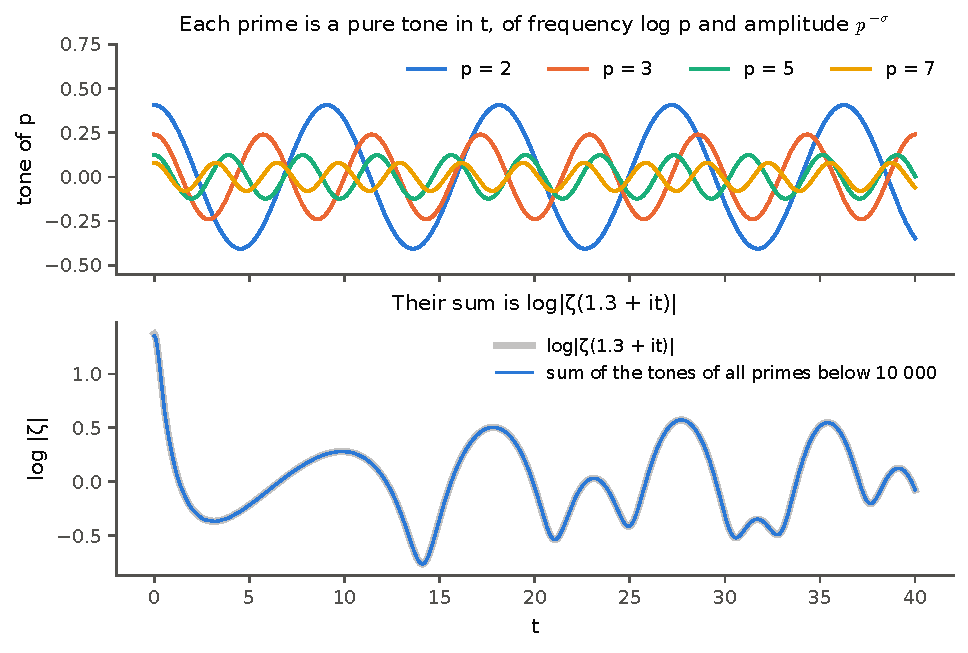
\includegraphics[width=0.86\textwidth]{lfun-tones}
  \caption{Top: the tones of the primes 2, 3, 5, 7. Bottom: the sum of the tones of all primes below $10^4$ against $\log|\zeta(1.3+it)|$.}
  \label{fig:tones}
\end{figure}

\section{On the critical line: a winding curve, and a bundle}

On $\mathrm{Re}\,s = \frac12$ the series no longer converges absolutely, but the function is still defined by continuation.
Plot $L(\tfrac12+it)$ in the complex plane as $t$ increases, and it traces a curve that winds through the origin at every zero (Figure~\ref{fig:curve}).
Draw the curves of the four $L$-functions of $\Q(\zeta_{12})$ together against $t$, and they form a bundle of curves winding along the $t$-axis (Figure~\ref{fig:bundle}).
Their product is the Dedekind zeta function of $\Q(\zeta_{12})$ (note~01).
The curves wind at different rates.
The number of zeros up to height $T$ is about $\frac{T}{2\pi}\log\frac{qT}{2\pi e}$ (Riemann--von Mangoldt \cite{Davenport}).
So the larger the modulus, the more zeros.
Below $t = 30$ the counts are 3, 10, 8 and 14 for $q = 1, 4, 3, 12$, against main terms $3.6$, $9.3$, $7.9$ and $14.6$.

\begin{figure}[ht]
  \centering
  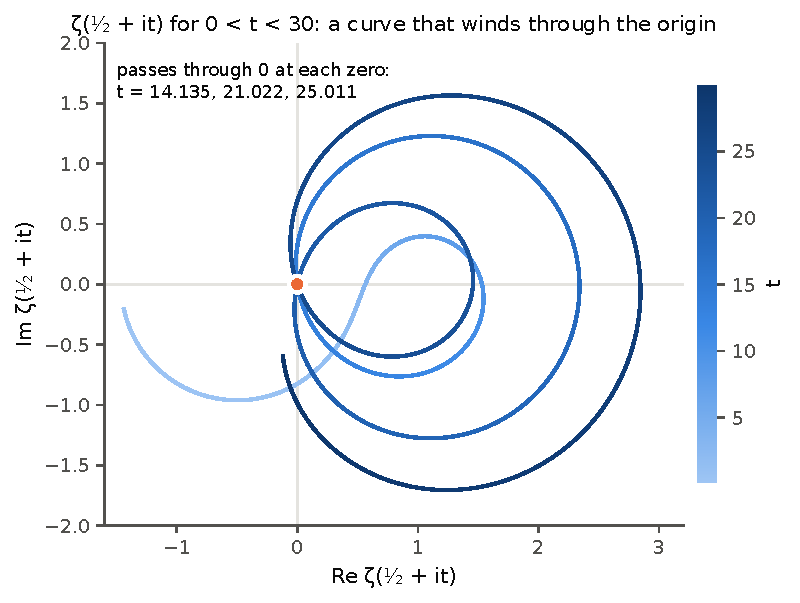
\includegraphics[width=0.66\textwidth]{lfun-critical-curve}
  \caption{$\zeta(\tfrac12+it)$ for $0<t<30$, shaded by $t$. The curve passes through the origin at the zeros $t = 14.135$, $21.022$, $25.011$.}
  \label{fig:curve}
\end{figure}

\begin{figure}[ht]
  \centering
  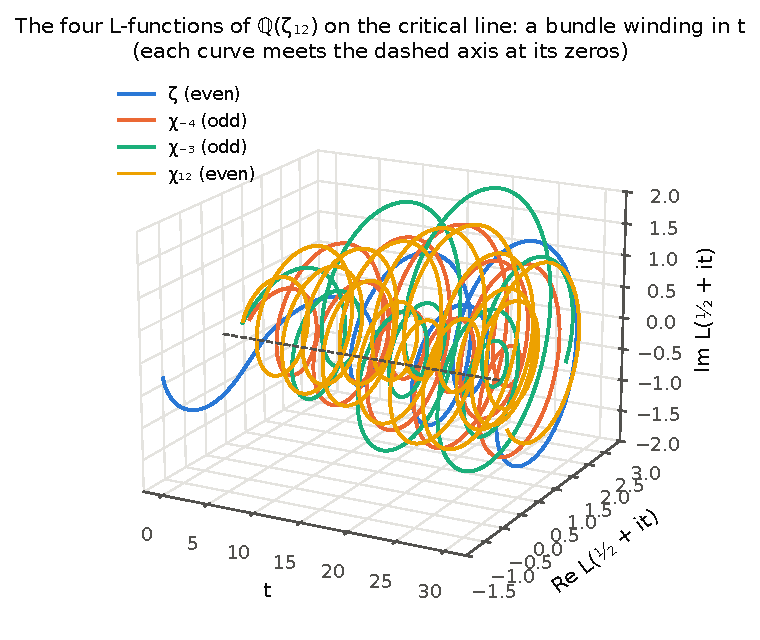
\includegraphics[width=0.8\textwidth]{lfun-bundle}
  \caption{The four $L$-functions of $\Q(\zeta_{12})$ on the critical line, plotted as curves $(t,\ \mathrm{Re}\,L,\ \mathrm{Im}\,L)$. Each meets the dashed $t$-axis at its zeros.}
  \label{fig:bundle}
\end{figure}

\section{Hardy's $Z$-function: seeing the zeros}

Let $\theta(t)$ be the argument of $(q/\pi)^{(s+a)/2}\Gamma(\frac{s+a}2)$ at $s=\frac12+it$.
Then $Z(t) = e^{i\theta(t)}L(\tfrac12+it,\chi)$ is real when the root number is~1, because the functional equation makes $\Lambda(\tfrac12+it)$ real.
A sign change of $Z$ is a zero of $L$ exactly on the critical line.
This is how zeros on the line are found and certified \cite{Titchmarsh}.
Figure~\ref{fig:hardy} shows the four $Z$-functions.
The script finds every sign change below $t=30$, refines each root, and checks that $|L| < 10^{-12}$ there.
The first zeros are $14.134725$ for $\zeta$, $6.020949$ for $\chi_{-4}$, $8.039737$ for $\chi_{-3}$ and $3.804628$ for $\chi_{12}$.
Sign changes show that these zeros are on the line.
Showing that there are no others below $t=30$ needs a count, by Turing's method, which this note does not do.

\begin{figure}[ht]
  \centering
  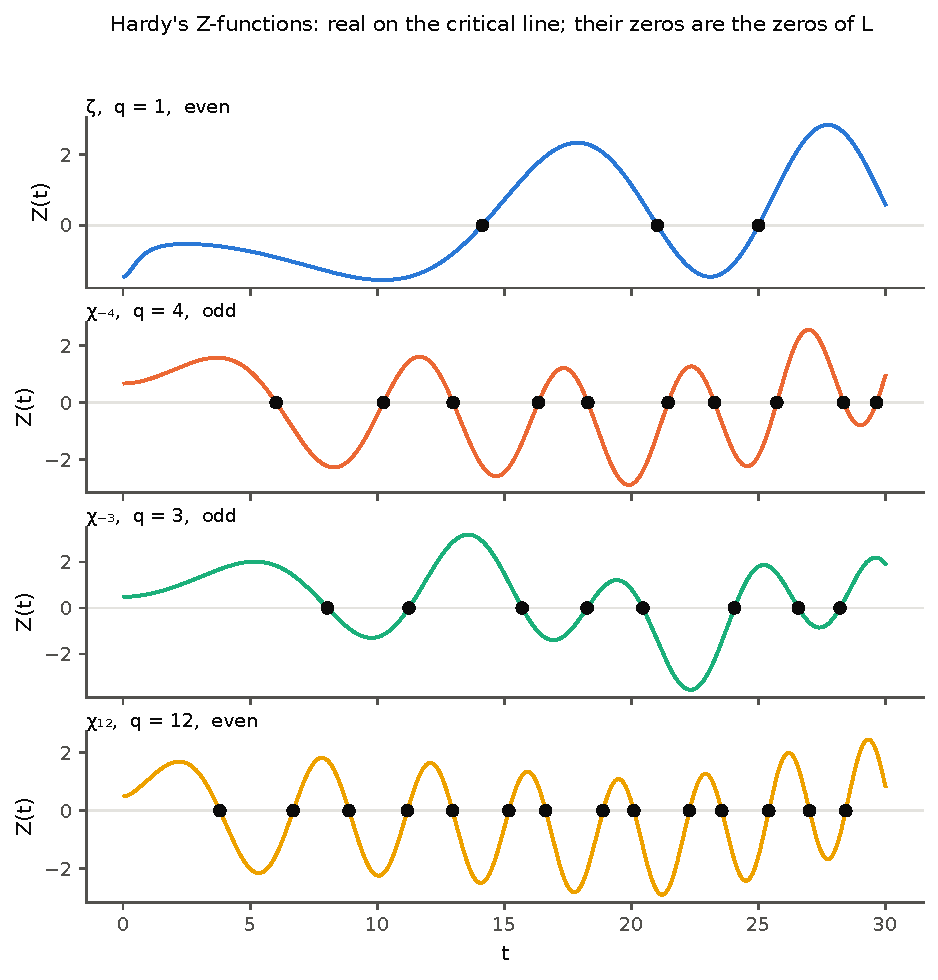
\includegraphics[width=0.86\textwidth]{lfun-hardy}
  \caption{Hardy's $Z$-functions of the four $L$-functions of $\Q(\zeta_{12})$, with their zeros below $t=30$.}
  \label{fig:hardy}
\end{figure}

\section{Parity: the first rung of chirality}

The parity $a$ sets the gamma factor, $\Gamma(s/2)$ or $\Gamma((s+1)/2)$, and with it the shape of $\theta(t)$.
For the character of a quadratic field, $\chi_D(-1)$ is the sign of $D$.
\begin{itemize}
\item The characters of imaginary fields are odd ($a=1$), like $\chi_{-4}$ and $\chi_{-3}$ for the Gaussian and Eisenstein fields.
In these fields complex conjugation is a non-trivial symmetry.
\item The characters of real fields are even ($a=0$), like $\chi_{12}$ for $\Q(\sqrt3)$, and so is $\zeta$.
\end{itemize}
Note~06 proposes this parity as the first rung of a ladder of handedness that continues through modular forms to the Standard Model.

\paragraph{What the pictures are not.}
The curves of Figures~\ref{fig:curve} and~\ref{fig:bundle} are not geodesics.
A precise geodesic picture of arithmetic is Selberg's.
The closed geodesics on the modular surface play the role of primes, their lengths are $2\log$ of units of real quadratic fields, and the shortest belongs to the golden ratio (note~05).

\section*{Status of the statements}

\begin{center}
\small
\begin{tabular}{@{}p{0.62\textwidth}l@{}}
\toprule
Statement & Grade\\
\midrule
Euler product, continuation, functional equation, root number & \gradeClassical\\
Prime tones reproduce $\log|\zeta(1.3+it)|$ to 1.3\% & \gradeComputed\\
$Z$ real; listed zeros on the line, $|L|<10^{-12}$; counts against Riemann--von Mangoldt & \gradeComputed\\
All non-trivial zeros on the critical line (GRH) & \gradeOpen\\
\bottomrule
\end{tabular}
\end{center}

\begin{thebibliography}{9}
\bibitem{Davenport} H.~Davenport, \emph{Multiplicative Number Theory}, 3rd ed., Springer, 2000.
\bibitem{Edwards} H.~M. Edwards, \emph{Riemann's Zeta Function}, Academic Press, 1974.
\bibitem{Titchmarsh} E.~C. Titchmarsh, \emph{The Theory of the Riemann Zeta-Function}, 2nd ed., revised by D.~R. Heath-Brown, Oxford University Press, 1986.
\end{thebibliography}

\end{document}
